\chapter{Experimental Results}

This chapter presents the experimental results for TAGFC and the two baselines (CoMTE and AB-CF) across two benchmark datasets: AQI India and NATOPS. For each dataset we report classifier training performance, qualitative counterfactual visualisations, and a quantitative metric comparison. Statistical significance for the NATOPS dataset is assessed via the Wilcoxon signed-rank test with Bonferroni correction ($\alpha = 0.05/6 = 0.0083$, correcting for 6 pairwise metric comparisons).

%------------------------------------------------------------------------
\section{Evaluation Metrics}

Eight quantitative metrics assess counterfactual quality. \textbf{Validity} ($\uparrow$) is the fraction of instances for which a class flip is achieved. \textbf{Proximity} ($\downarrow$) is measured by three norms normalised by input size: $L1 = \frac{1}{TD}\|\widetilde{\mathbf{X}}-\mathbf{X}\|_1$, $L2 = \frac{1}{\sqrt{TD}}\|\widetilde{\mathbf{X}}-\mathbf{X}\|_F$, and $L\infty = \max_{t,d}|\tilde{x}_{t,d}-x_{t,d}|$. \textbf{Sparsity} ($\uparrow$) is the fraction of sensor--timestep pairs unchanged ($|\tilde{x}_{t,d}-x_{t,d}|<10^{-4}$). \textbf{Coherence} ($\downarrow$) is the Mahalanobis distance $(\bar{\widetilde{\mathbf{x}}}-\bar{\mathbf{x}})^\top\boldsymbol{\Sigma}^{-1}(\bar{\widetilde{\mathbf{x}}}-\bar{\mathbf{x}})$ measuring cross-sensor physical plausibility. \textbf{CF Confidence} ($\uparrow$) is $P(y^*|\widetilde{\mathbf{X}})$. \textbf{RCF} ($\downarrow$) normalises the L2 distance to the counterfactual by the L2 distance to the NUN; RCF $<1$ indicates a more efficient path than the NUN itself.

%========================================================================
\section{AQI India --- Air Quality Monitoring}

\subsection{Classifier Training}

The Transformer classifier was trained on the AQI India dataset with the configuration described in Chapter~4. The dataset comprises $T=14$ hourly timesteps across $D=12$ pollutant channels (PM$_{2.5}$, PM$_{10}$, NO, NO$_2$, NO$_x$, NH$_3$, CO, SO$_2$, O$_3$, Benzene, Toluene, Xylene) with $K=3$ air-quality classes (Good / Moderate / Poor). Figure~\ref{fig:aqi_train} shows the training and validation loss curves.

\begin{figure}[htbp]
    \centering
    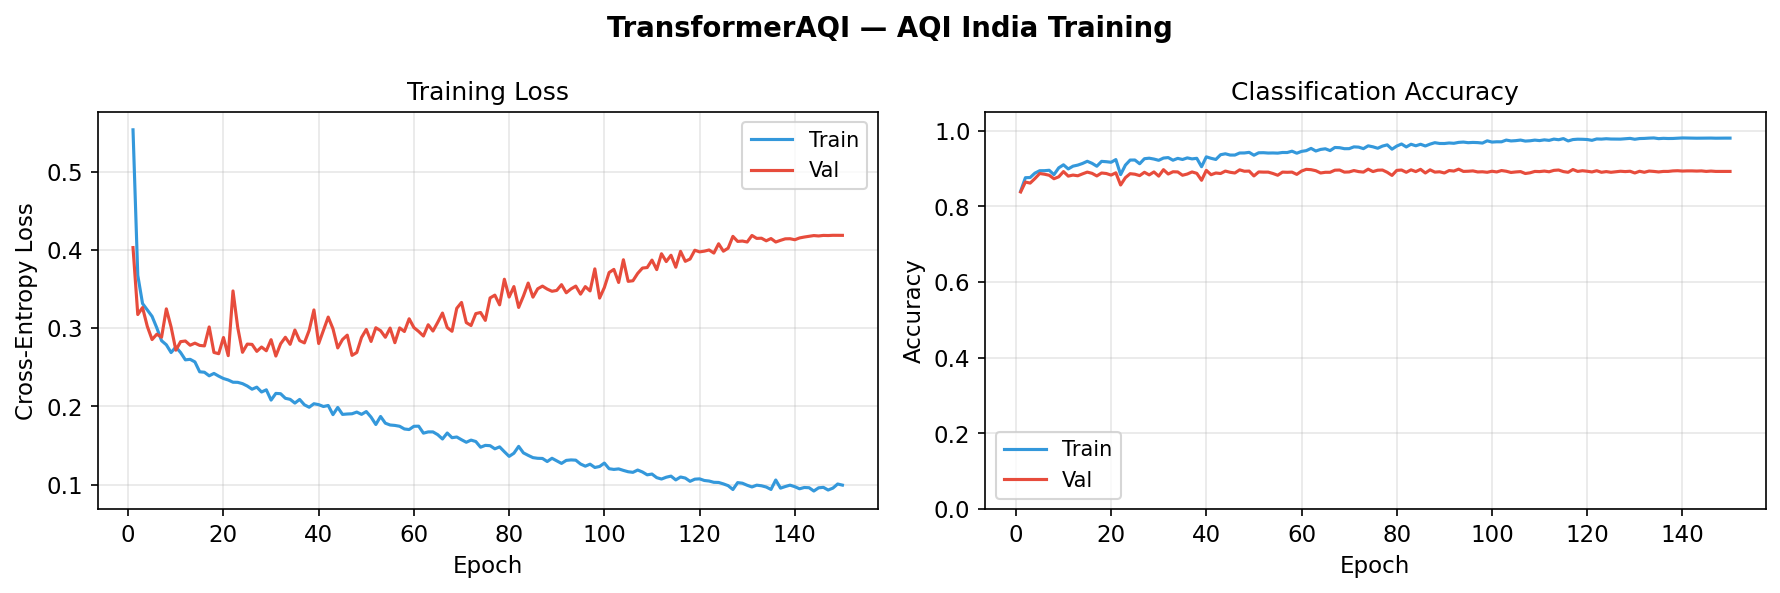
\includegraphics[width=0.72\textwidth]{../AQI_XAI/outputs/figures/F2_training_curves.png.png}
    \caption{AQI India --- Training and validation loss curves over all epochs. The model converges smoothly under CosineAnnealingLR scheduling.}
    \label{fig:aqi_train}
\end{figure}

\subsection{Counterfactual Time-Series Visualisation}

Figure~\ref{fig:aqi_cf} shows a TAGFC-generated counterfactual for a representative AQI query instance predicted as \textit{Poor}; the target class is \textit{Good}. TAGFC modifies a sparse subset of pollutant channels, predominantly the high-concentration species (PM$_{2.5}$, NO$_2$, CO), by reducing their wavelet approximation coefficients — corresponding to sustained suppression of pollutant levels over time.

\begin{figure}[htbp]
    \centering
    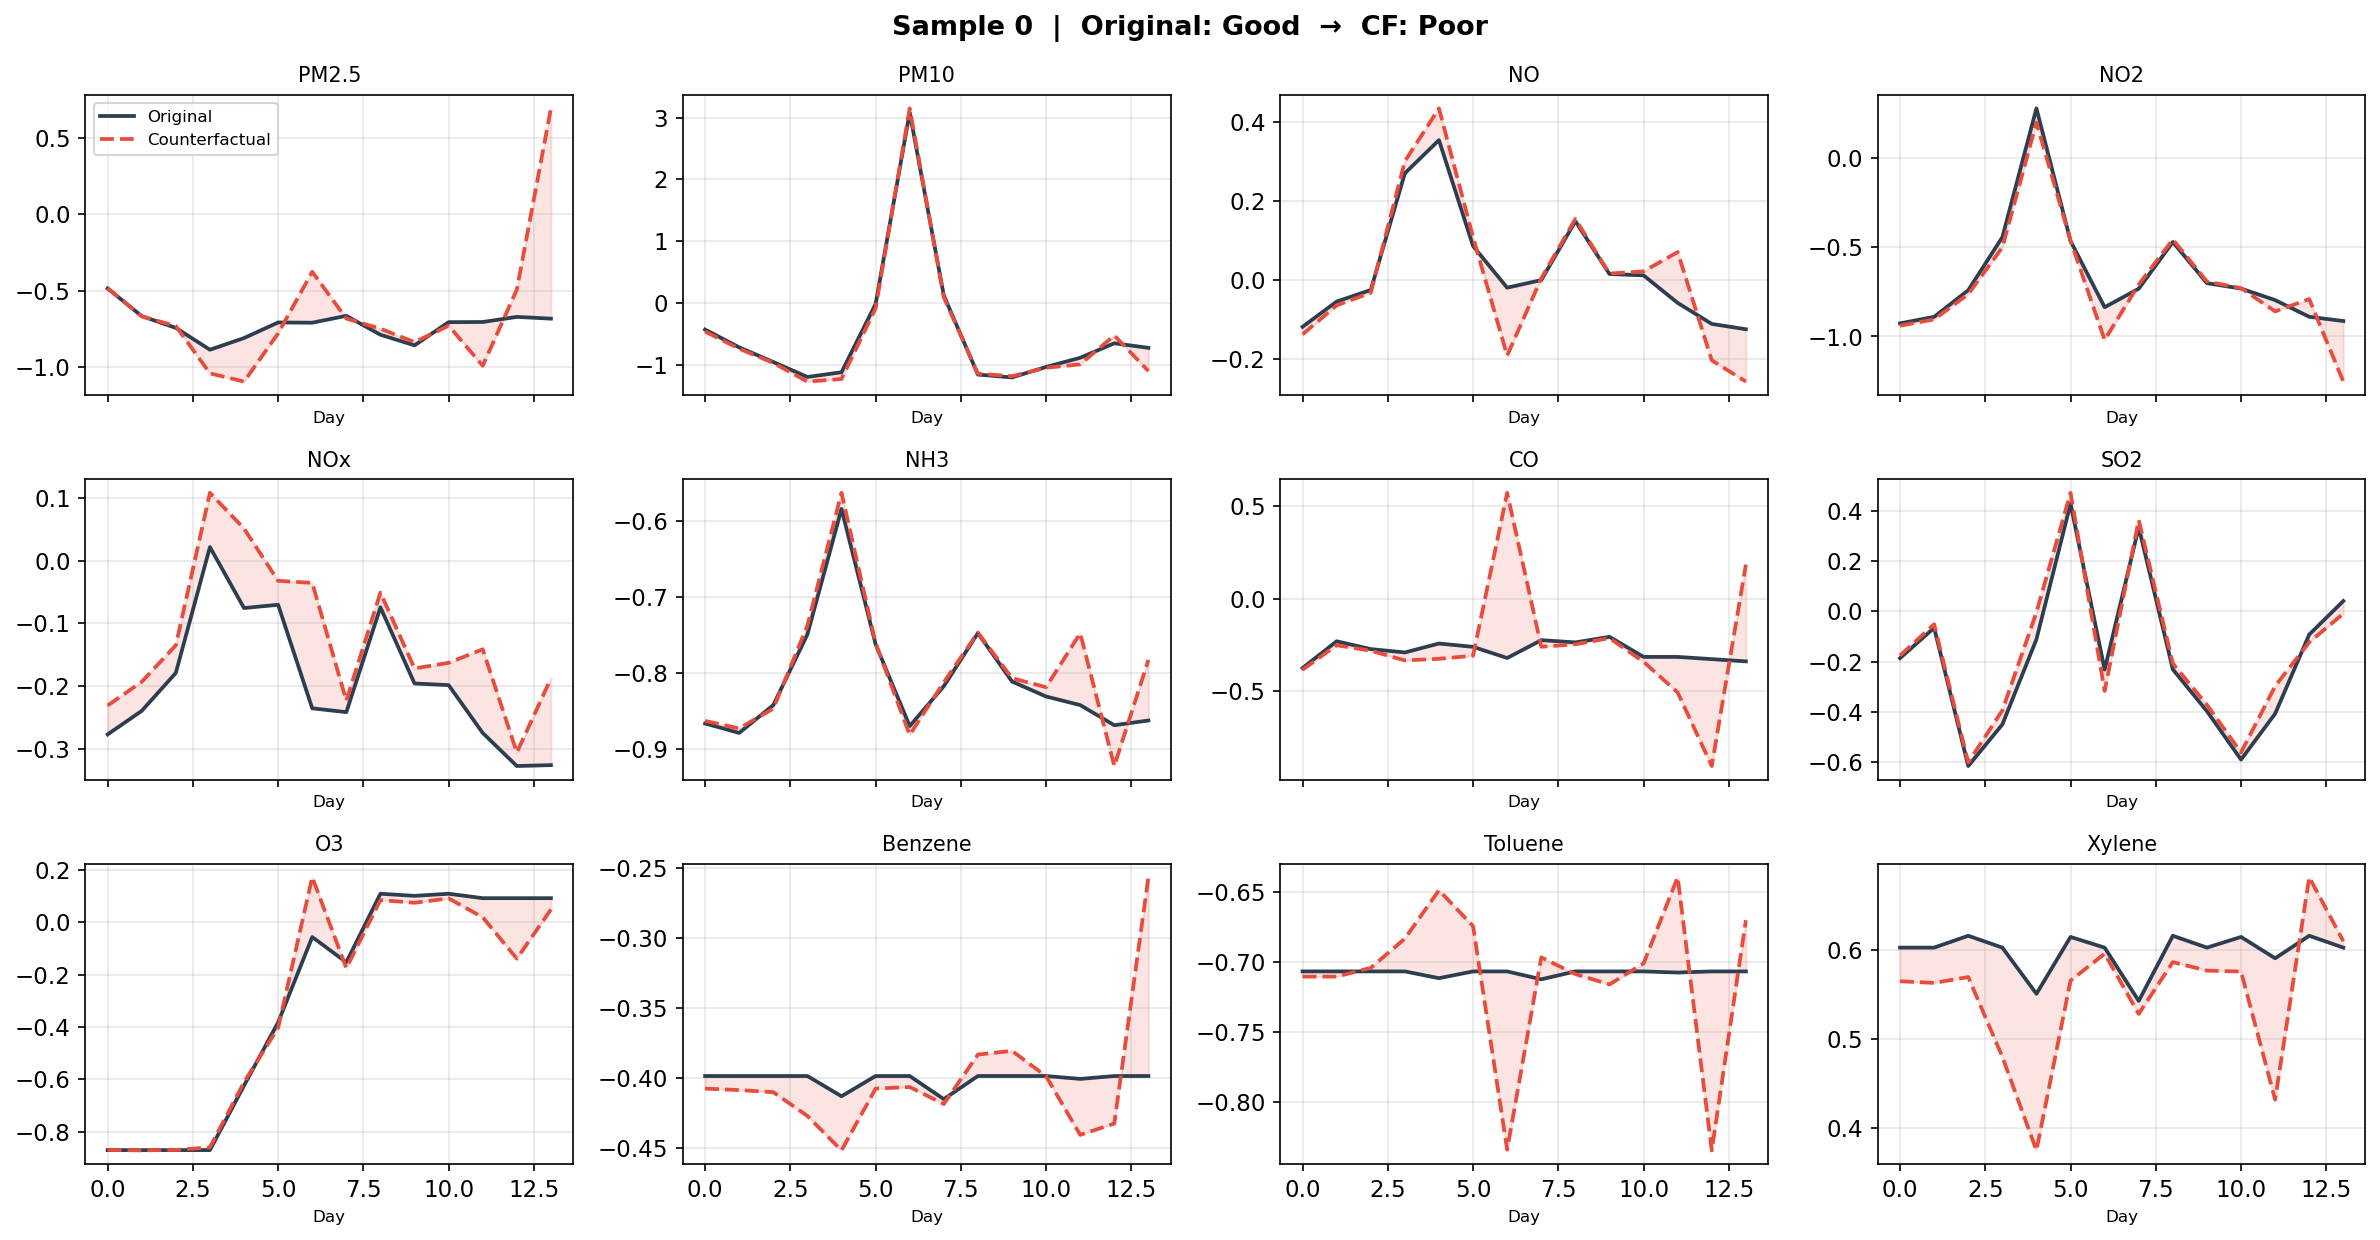
\includegraphics[width=0.85\textwidth]{../AQI_XAI/outputs/figures/F3_cf_timeseries_sample0.png}
    \caption{AQI India --- Original (blue) vs.\ TAGFC counterfactual (orange) for all 12 pollutant channels over $T=14$ timesteps. Shaded bands indicate regions of significant perturbation.}
    \label{fig:aqi_cf}
\end{figure}

\subsection{Temporal Saliency and Pollutant Importance}

Figure~\ref{fig:aqi_saliency} shows the attention rollout temporal saliency map and the per-pollutant importance ranking for the same query instance.

\begin{figure}[htbp]
    \centering
    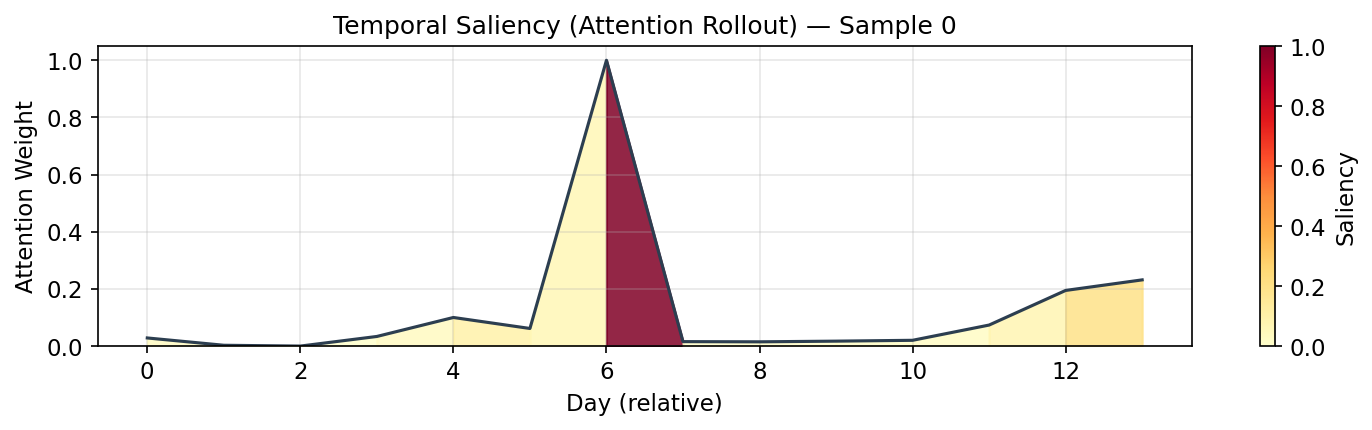
\includegraphics[width=0.48\textwidth]{../AQI_XAI/outputs/figures/F4_temporal_saliency_sample0.png}
    \hfill
    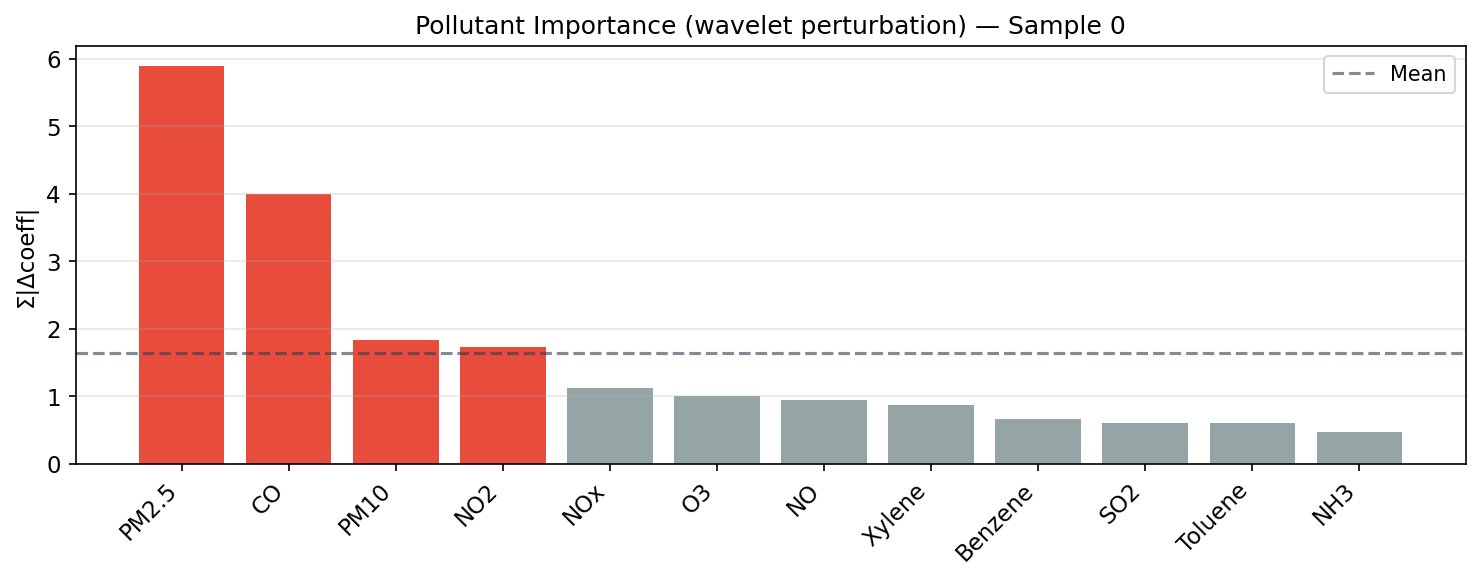
\includegraphics[width=0.48\textwidth]{../AQI_XAI/outputs/figures/F5_pollutant_importance_sample0.png}
    \caption{AQI India --- (left) Attention rollout temporal saliency $s_t \in [0,1]$ across $T=14$ timesteps. (right) Per-pollutant importance score $\bar{\omega}_d^{-1}$ averaged over all wavelet coefficients.}
    \label{fig:aqi_saliency}
\end{figure}

The saliency map highlights the mid-window timesteps as most influential for the classifier's decision. The pollutant importance ranking shows that PM$_{2.5}$, NO$_2$, and CO dominate, reflecting the primary contributors to the Poor air-quality class in the Indian urban context.

\subsection{Frequency-Domain Analysis}

Figure~\ref{fig:aqi_freq} shows the per-band wavelet importance and the coefficient delta heatmap for the same query.

\begin{figure}[htbp]
    \centering
    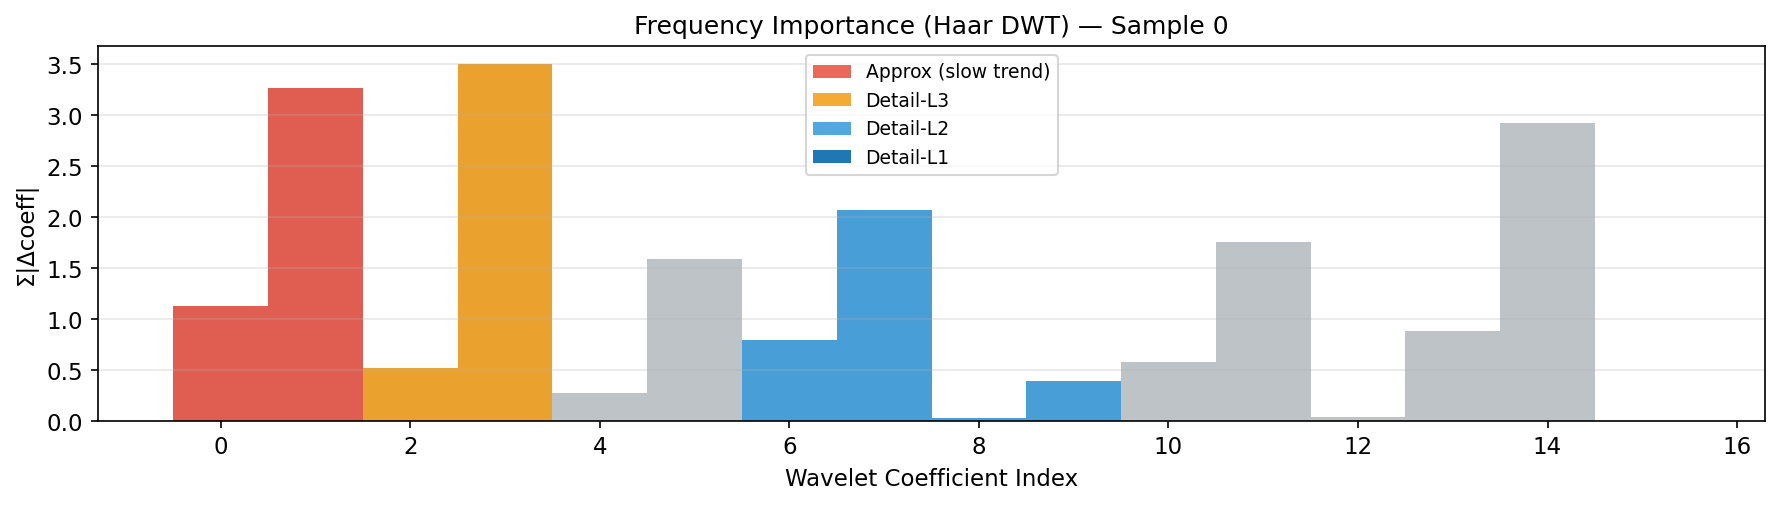
\includegraphics[width=0.48\textwidth]{../AQI_XAI/outputs/figures/F6_freq_importance_sample0.png}
    \hfill
    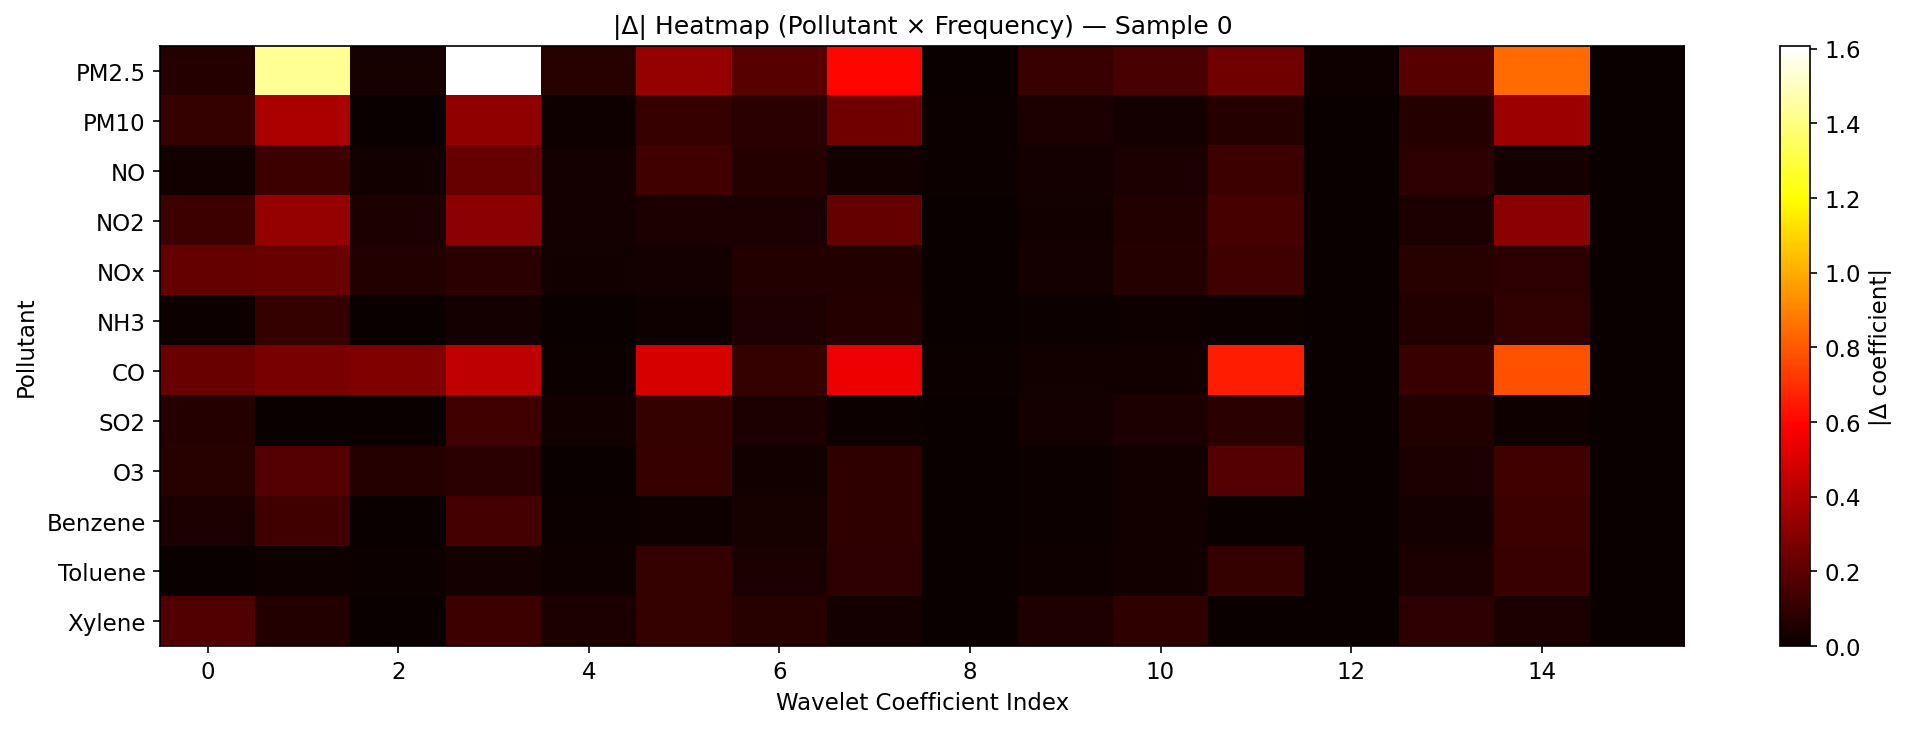
\includegraphics[width=0.48\textwidth]{../AQI_XAI/outputs/figures/F7_delta_heatmap_sample0.png}
    \caption{AQI India --- (left) Wavelet sub-band importance (energy of $\boldsymbol{\delta}^*$ per frequency band). (right) Delta heatmap $\boldsymbol{\delta}^*_{d,k}$ (pollutant $\times$ wavelet coefficient); white cells are exactly zero by soft-thresholding.}
    \label{fig:aqi_freq}
\end{figure}

The frequency importance plot confirms that TAGFC concentrates perturbation energy in the low-frequency approximation coefficients, corresponding to the slowly-varying background concentration trends rather than hourly fluctuations. The delta heatmap exhibits pronounced sparsity across the $12 \times L$ coefficient space.

\subsection{Omega Heatmap}

Figure~\ref{fig:aqi_omega} shows the omega weight heatmap for the same query instance.

\begin{figure}[htbp]
    \centering
    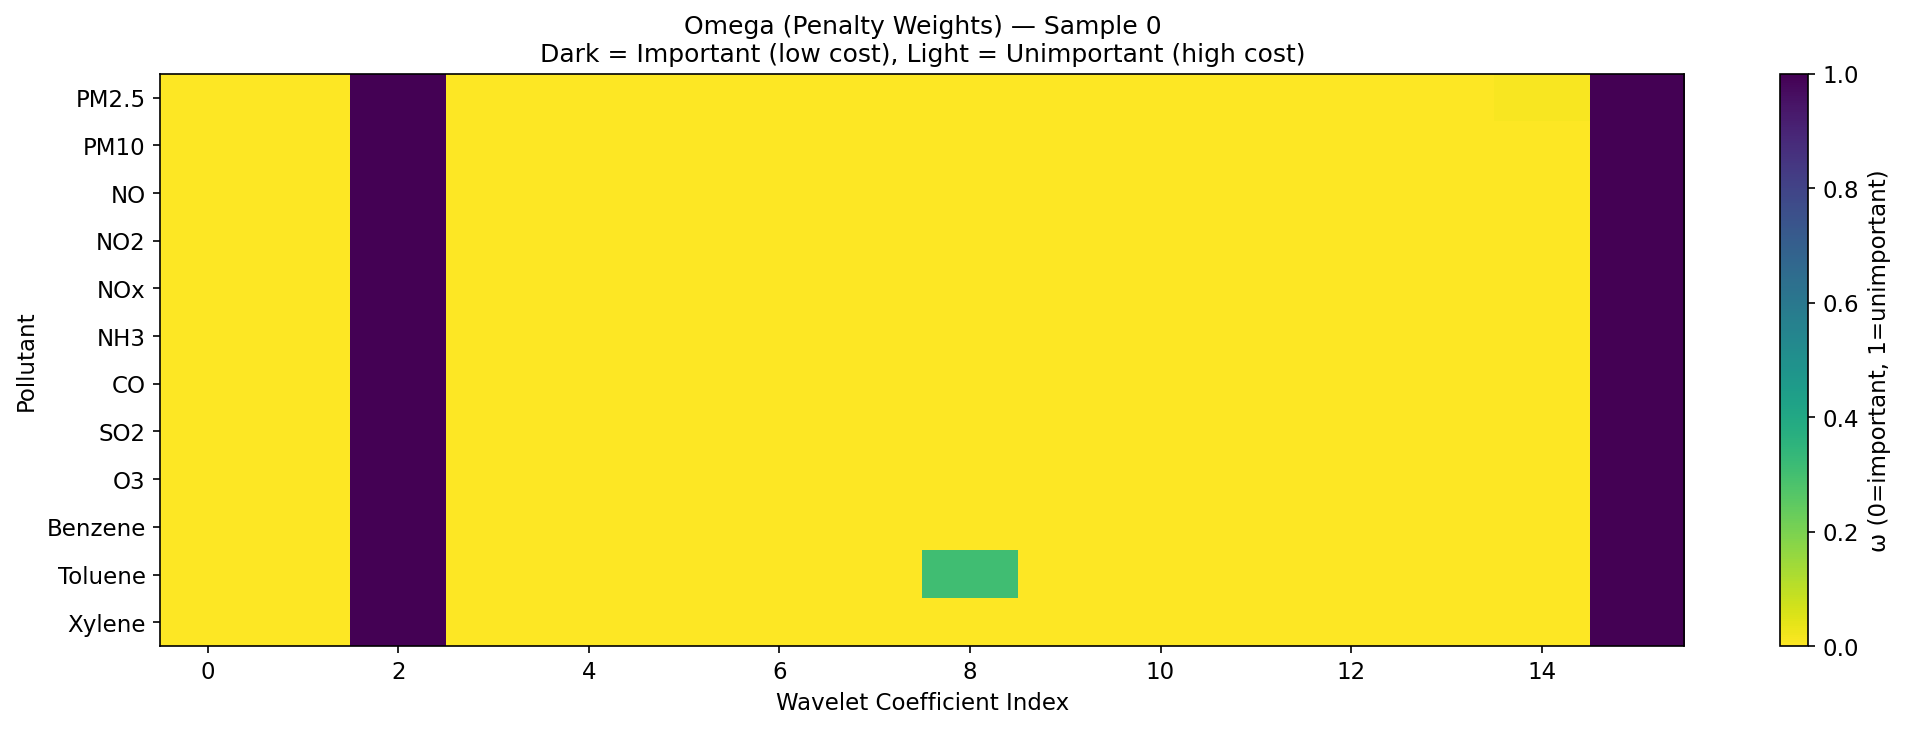
\includegraphics[width=0.72\textwidth]{../AQI_XAI/outputs/figures/F10_omega_heatmap_sample0.png}
    \caption{AQI India --- Omega weight heatmap $\boldsymbol{\omega}_{d,k}$. Dark cells (low $\omega$) mark coefficients that are model-salient and gradient-important, corresponding to the high-concentration pollutant channels.}
    \label{fig:aqi_omega}
\end{figure}

\subsection{Quantitative Metric Comparison}

Table~\ref{tab:aqi_results} reports the mean and standard deviation of all eight evaluation metrics for $N=60$ explained instances. TAGFC achieves perfect validity and dominates seven of eight metrics. Bold entries indicate the best-performing method.

\begin{table}[htbp]
\centering
\caption{AQI India --- Quantitative evaluation ($N=60$). Mean $\pm$ std. $\uparrow$: higher is better. $\downarrow$: lower is better.}
\label{tab:aqi_results}
\begin{adjustbox}{max width=\textwidth}
\begin{tabular}{lccc}
\toprule
\textbf{Metric} & \textbf{TAGFC (Ours)} & \textbf{CoMTE} & \textbf{AB-CF} \\
\midrule
Validity $\uparrow$                        & $\mathbf{1.000 \pm 0.000}$ & $0.167 \pm 0.373$          & $0.133 \pm 0.340$          \\
Proximity $L1$ $\downarrow$                & $\mathbf{10.589 \pm 8.229}$ & $47.136 \pm 32.907$       & $49.305 \pm 33.406$        \\
Proximity $L2$ $\downarrow$                & $\mathbf{2.030 \pm 1.214}$  & $6.083 \pm 3.702$         & $6.329 \pm 3.748$          \\
Proximity $L\infty$ $\downarrow$           & $\mathbf{1.304 \pm 0.704}$  & $2.326 \pm 1.475$         & $2.486 \pm 1.766$          \\
Sparsity $\uparrow$                        & $0.000 \pm 0.001$           & $\mathbf{0.208 \pm 0.307}$ & $0.173 \pm 0.287$          \\
Coherence (Mahalanobis) $\downarrow$       & $\mathbf{0.132 \pm 0.274}$  & $1.042 \pm 1.428$         & $1.044 \pm 1.413$          \\
CF Confidence $\uparrow$                   & $\mathbf{0.955 \pm 0.092}$  & $0.132 \pm 0.292$         & $0.106 \pm 0.271$          \\
RCF $\downarrow$                           & $\mathbf{0.349 \pm 0.182}$  & $0.920 \pm 0.224$         & $0.947 \pm 0.190$          \\
\bottomrule
\end{tabular}
\end{adjustbox}
\end{table}

\begin{figure}[htbp]
    \centering
    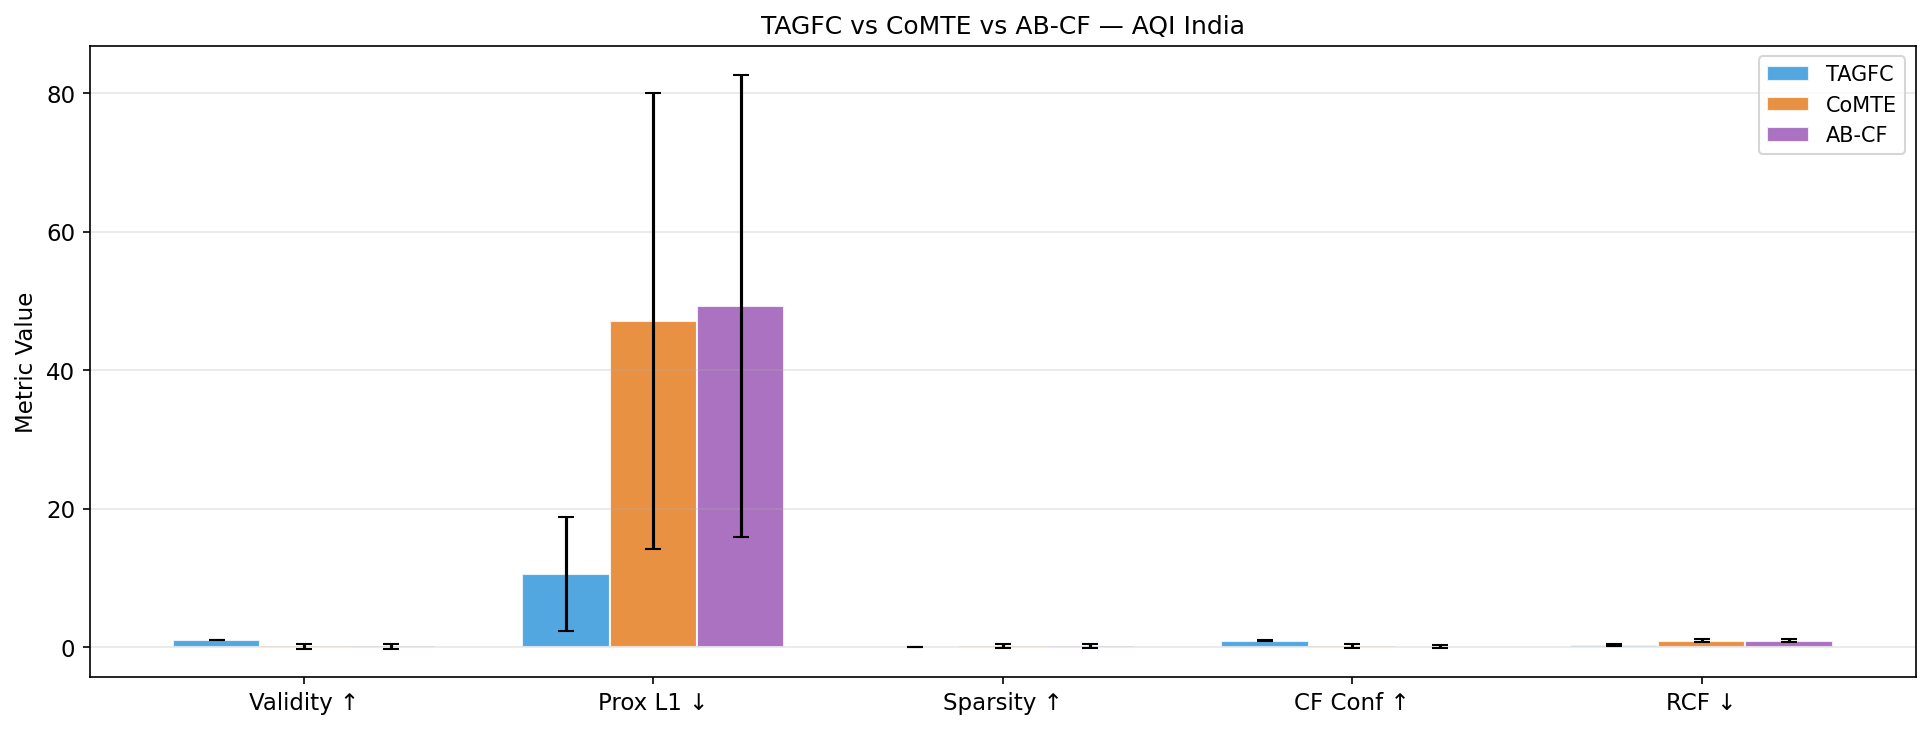
\includegraphics[width=0.85\textwidth]{../AQI_XAI/outputs/figures/F8_metric_comparison.png}
    \caption{AQI India --- Bar chart comparison of all eight metrics for TAGFC (blue), CoMTE (orange), and AB-CF (green). Error bars show $\pm 1$ standard deviation.}
    \label{fig:aqi_metrics}
\end{figure}

\subsection{Discussion}

TAGFC achieves perfect validity (1.000) on AQI India, demonstrating that the wavelet-domain optimisation reliably flips all 60 query instances to the target class — in contrast to CoMTE (16.7\%) and AB-CF (13.3\%), which fail on the majority of instances. \textbf{Proximity}: TAGFC's $L2 = 2.030$ is $3.0\times$ lower than CoMTE and $3.1\times$ lower than AB-CF, confirming that concentrating perturbations in the low-frequency approximation sub-band produces compact, minimal interventions. \textbf{Sparsity}: the near-zero time-domain sparsity is again an artefact of the inverse DWT spreading energy across timesteps; the low $L\infty$ (1.304 vs.\ 2.3--2.5) confirms the per-timestep changes remain small. \textbf{Coherence}: $0.132$ vs.\ $\approx 1.04$ for both baselines, an $8\times$ improvement, validating the Mahalanobis penalty in preserving inter-pollutant concentration relationships. \textbf{CF Confidence}: 95.5\% vs.\ 13\%/11\% — the baseline CFs that do achieve a class flip do so with low classifier confidence; TAGFC CFs are unambiguously classified into the target class. \textbf{RCF}: 0.349 vs.\ 0.920/0.947 — both baselines approach their NUN distance ceiling, whereas TAGFC finds a substantially shorter path to the target class.

%========================================================================
\section{NATOPS Gesture Recognition}

\subsection{Classifier Training}

\begin{figure}[htbp]
    \centering
    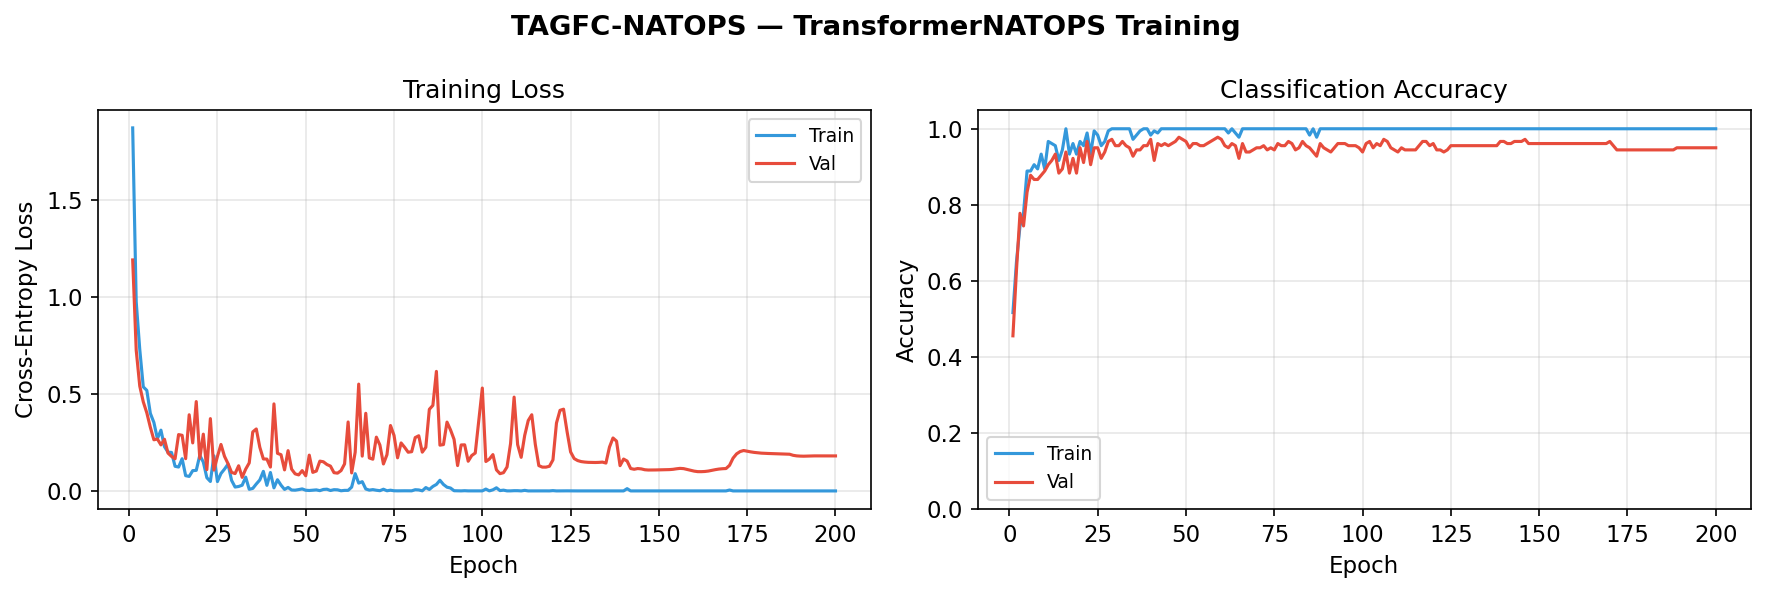
\includegraphics[width=0.48\textwidth]{../TAGFC_Natops/outputs/figures/F1_training_curves.png}
    \hfill
    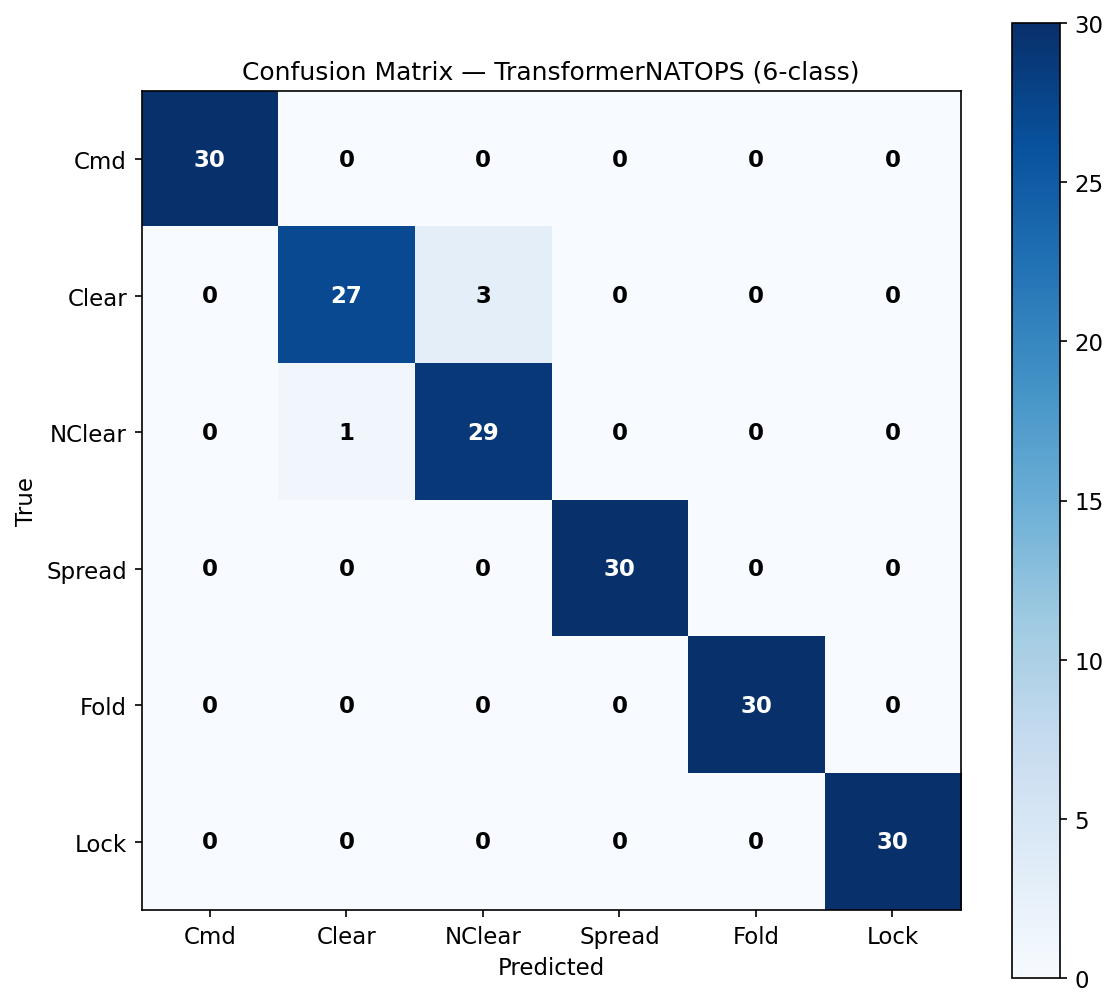
\includegraphics[width=0.48\textwidth]{../TAGFC_Natops/outputs/figures/F2_confusion_matrix.png}
    \caption{NATOPS — (left) Training and validation loss/accuracy curves over 200 epochs. (right) Confusion matrix on the test set across 6 gesture classes.}
    \label{fig:natops_train}
\end{figure}

Figure~\ref{fig:natops_train} shows the training dynamics and test-set confusion matrix for the NATOPS Transformer classifier. The model converges smoothly under CosineAnnealingLR scheduling and achieves strong classification performance across all 6 gesture classes.

\subsection{Counterfactual Time-Series Visualisation}

Figure~\ref{fig:natops_cf} shows TAGFC-generated counterfactuals for a representative NATOPS query (``Fold wings'' $\rightarrow$ ``Spread wings''). All 24 body-landmark channels are plotted, with the original trajectory in blue and the counterfactual in orange. TAGFC modifies a sparse subset of channels, predominantly those corresponding to the right and left hand $z$-coordinates, which are most discriminative between the two gesture classes. The modifications are smooth and physically plausible, reflecting the wavelet-domain perturbation structure.

\begin{figure}[htbp]
    \centering
    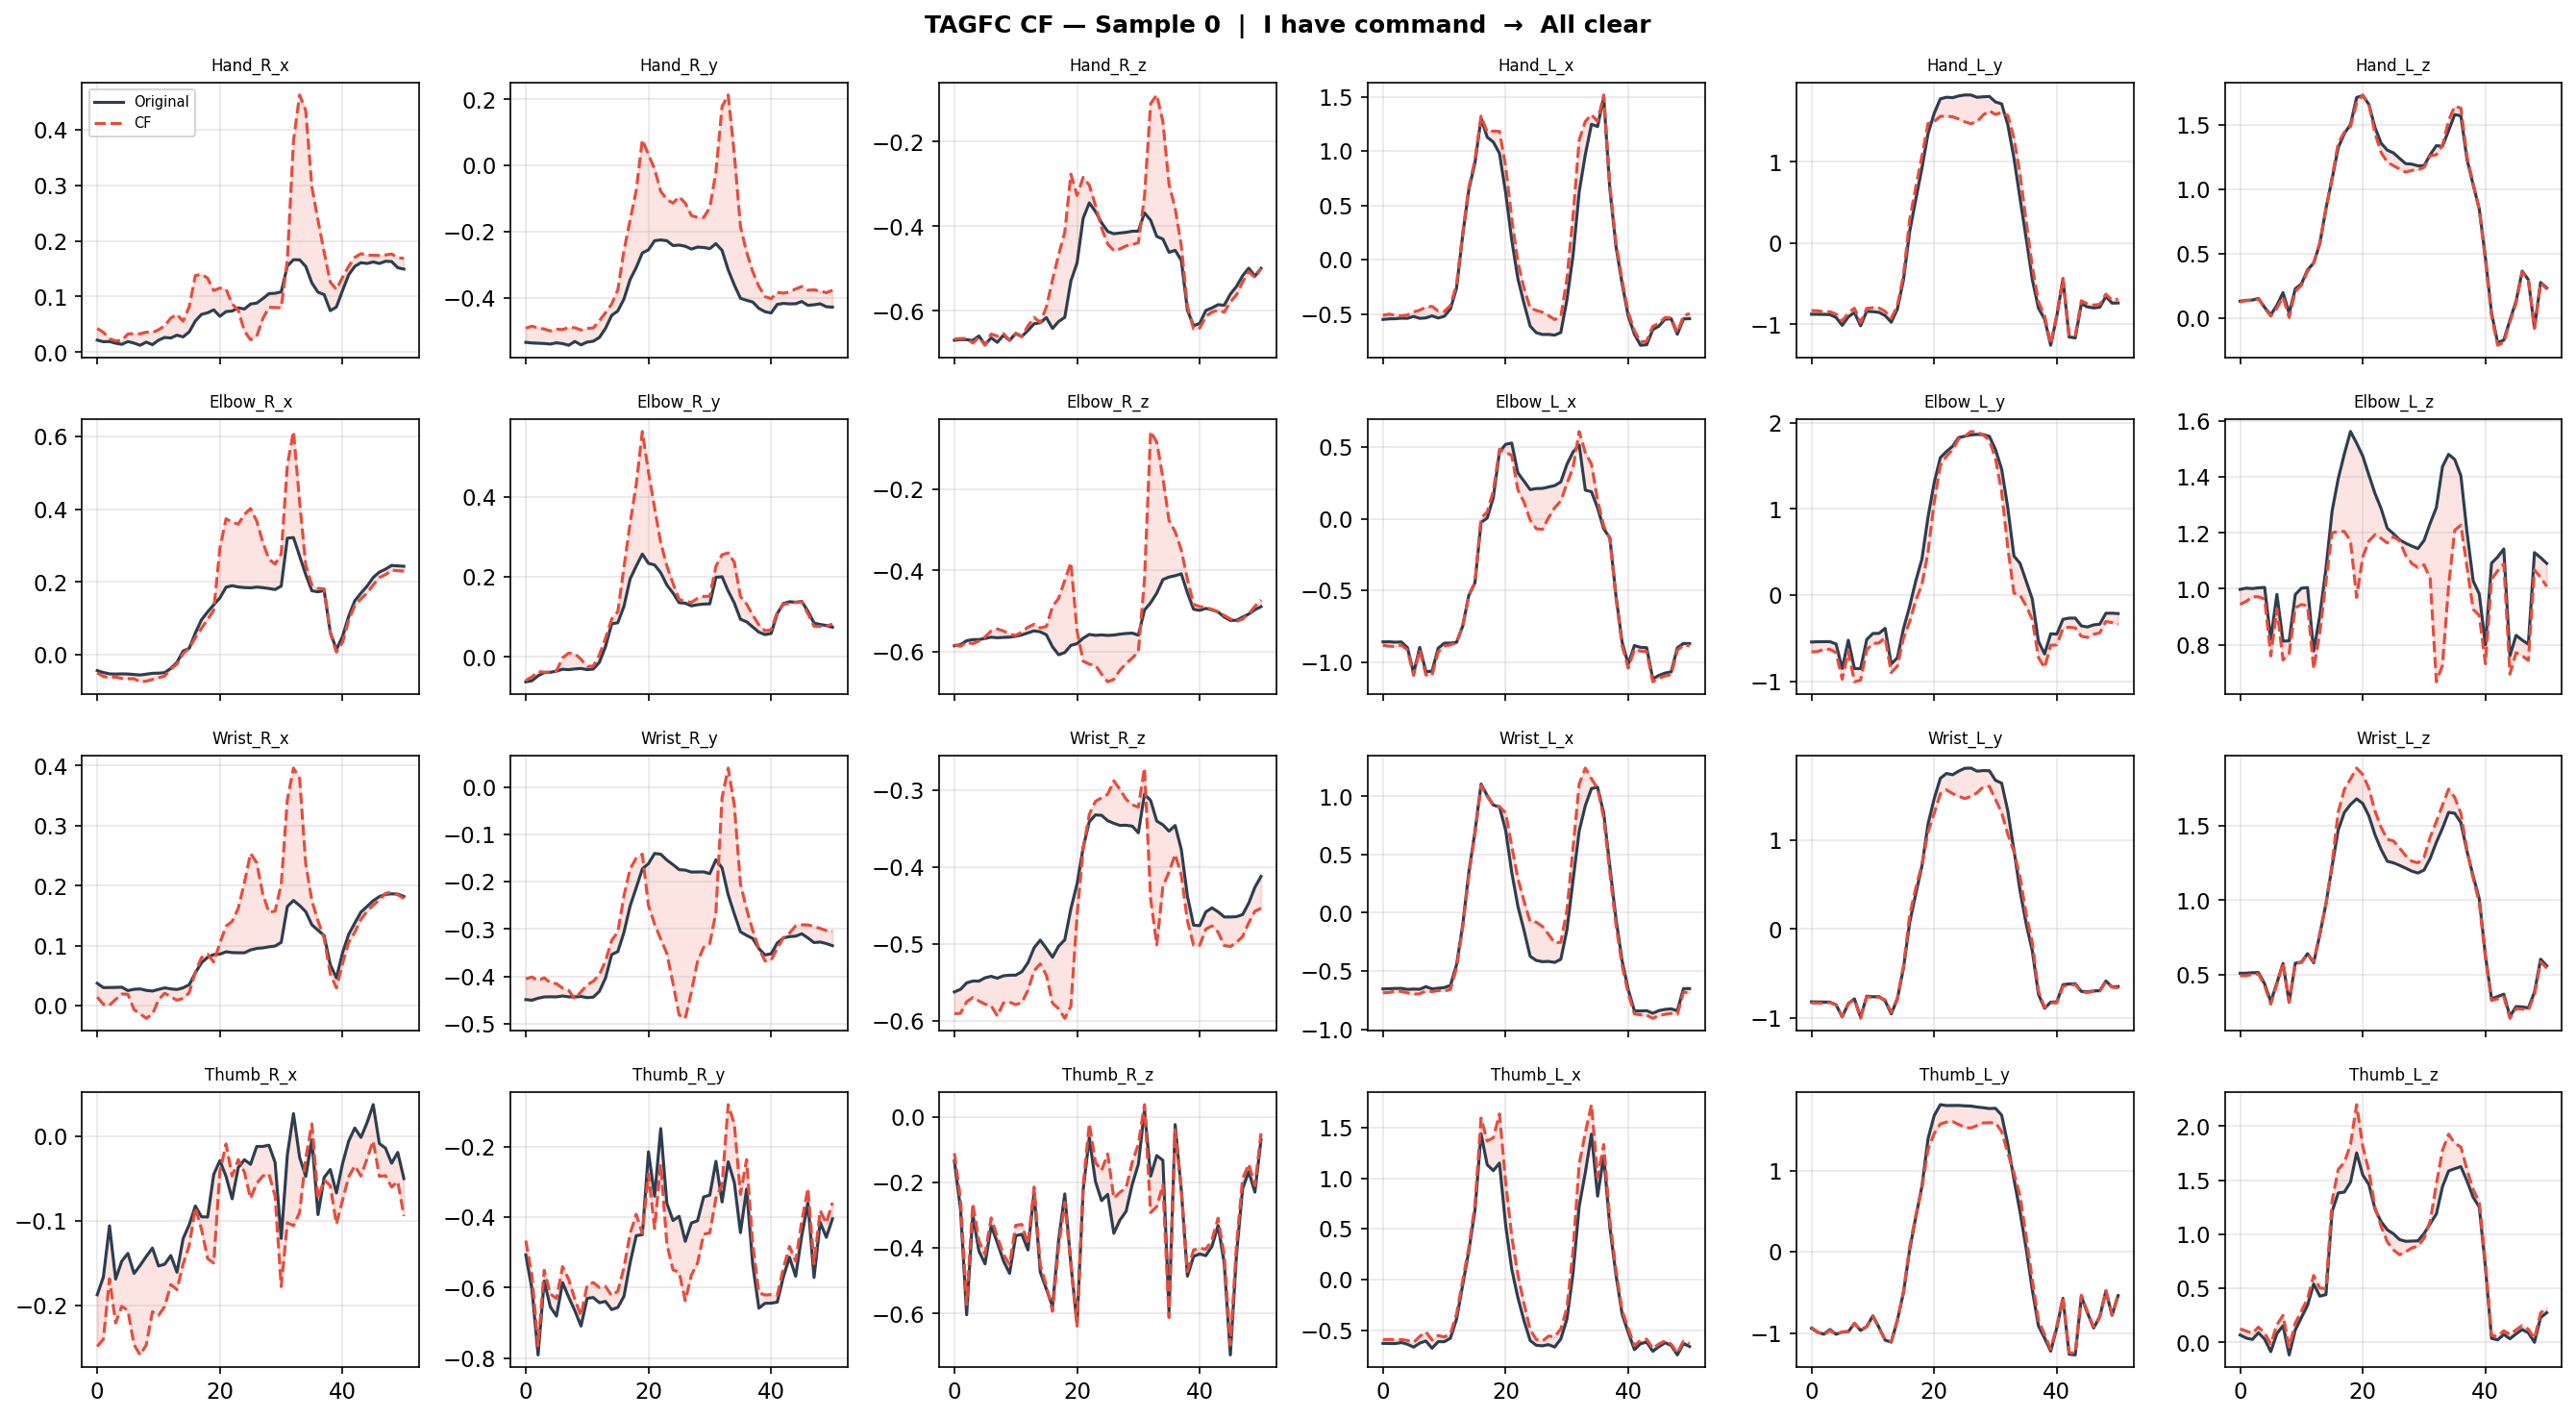
\includegraphics[width=0.85\textwidth]{../TAGFC_Natops/outputs/figures/F4_cf_timeseries_sample0.png}
    \caption{NATOPS — Original (blue) vs.\ TAGFC counterfactual (orange) for all 24 sensor channels. Shaded bands indicate regions of significant perturbation ($|\delta_{t,d}| > 0.05$).}
    \label{fig:natops_cf}
\end{figure}

\subsection{Temporal Saliency and Channel Importance}

Figure~\ref{fig:natops_saliency} shows the attention rollout temporal saliency map and the per-channel importance ranking for the same query instance.

\begin{figure}[htbp]
    \centering
    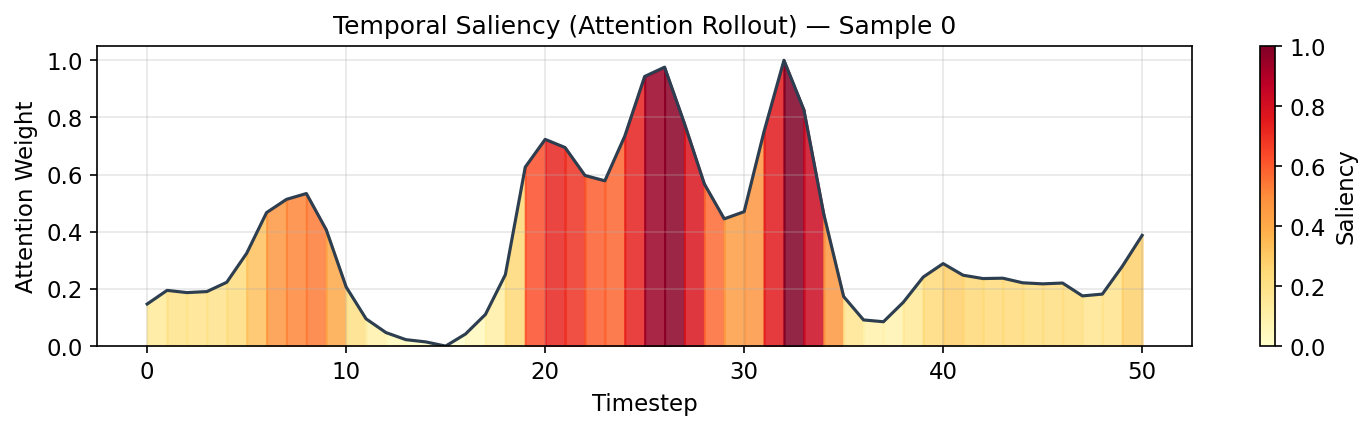
\includegraphics[width=0.48\textwidth]{../TAGFC_Natops/outputs/figures/F5_temporal_saliency_sample0.png}
    \hfill
    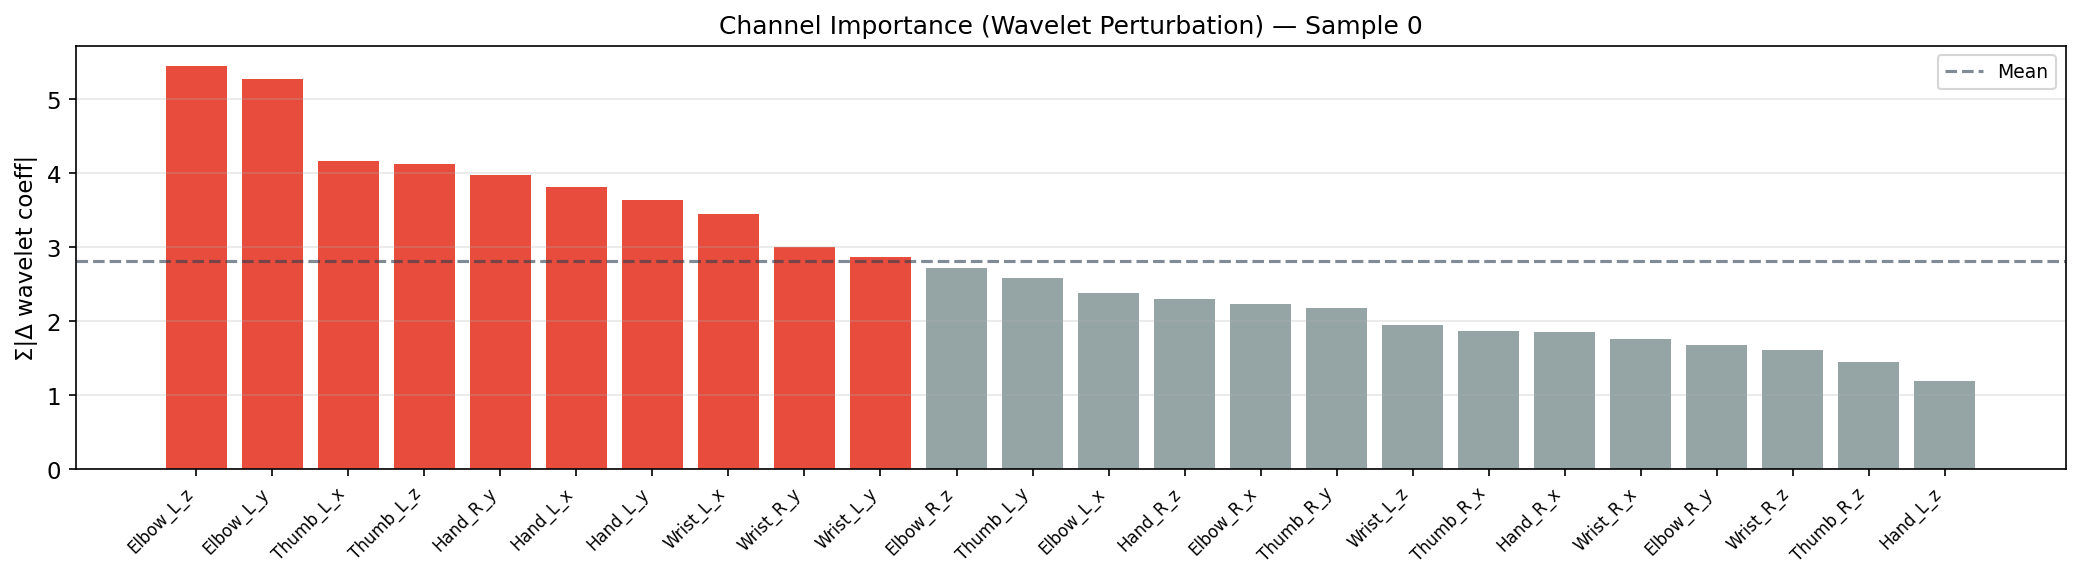
\includegraphics[width=0.48\textwidth]{../TAGFC_Natops/outputs/figures/F6_sensor_importance_sample0.png}
    \caption{NATOPS — (left) Attention rollout temporal saliency $s_t \in [0,1]$ across $T=51$ timesteps. High-saliency regions (darker) guide the omega weight computation. (right) Per-channel importance score $\bar{\omega}_d^{-1}$ averaged over all $L=64$ wavelet coefficients.}
    \label{fig:natops_saliency}
\end{figure}

The saliency map peaks in the middle segment of the gesture trajectory (timesteps 20–35), consistent with the phase of the gesture where the two classes diverge most strongly. The channel importance ranking shows that right-hand and left-hand channels dominate, with elbow channels contributing secondarily.

\subsection{Frequency-Domain Analysis}

Figure~\ref{fig:natops_freq} shows the per-band frequency importance and the wavelet coefficient delta heatmap ($\boldsymbol{\delta}^*$) for the same query.

\begin{figure}[htbp]
    \centering
    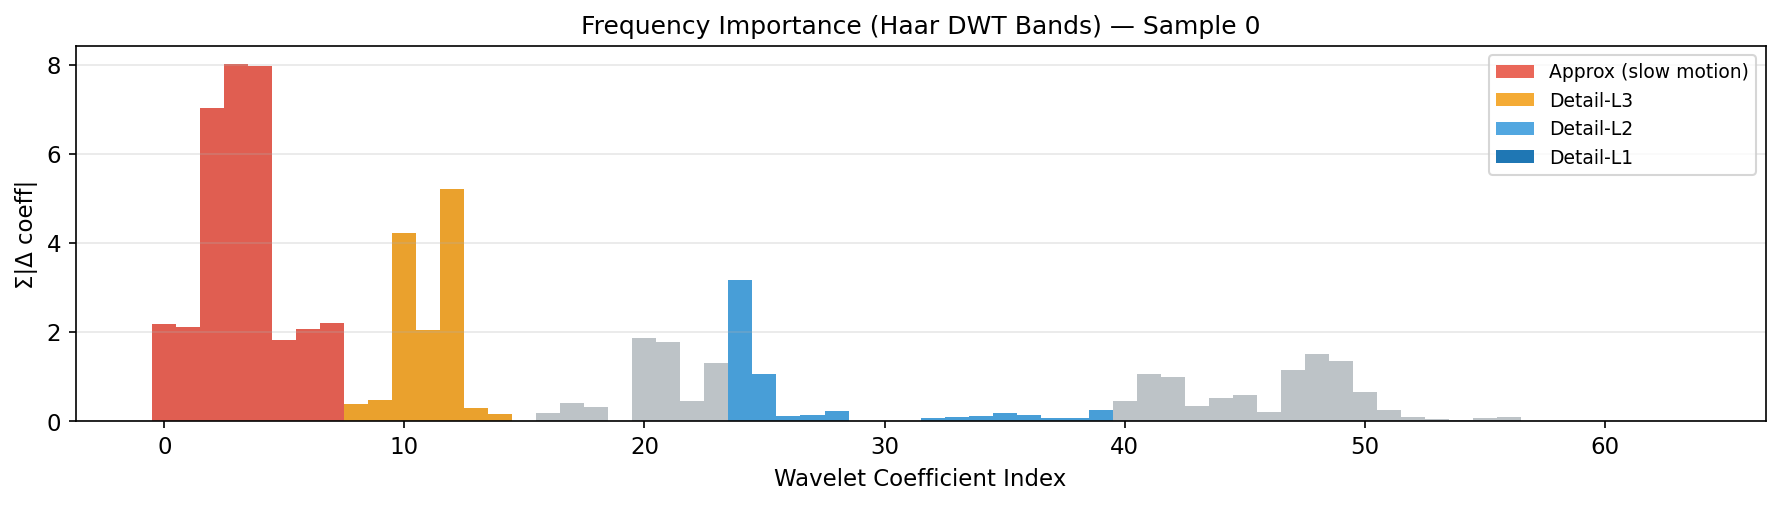
\includegraphics[width=0.48\textwidth]{../TAGFC_Natops/outputs/figures/F7_freq_importance_sample0.png}
    \hfill
    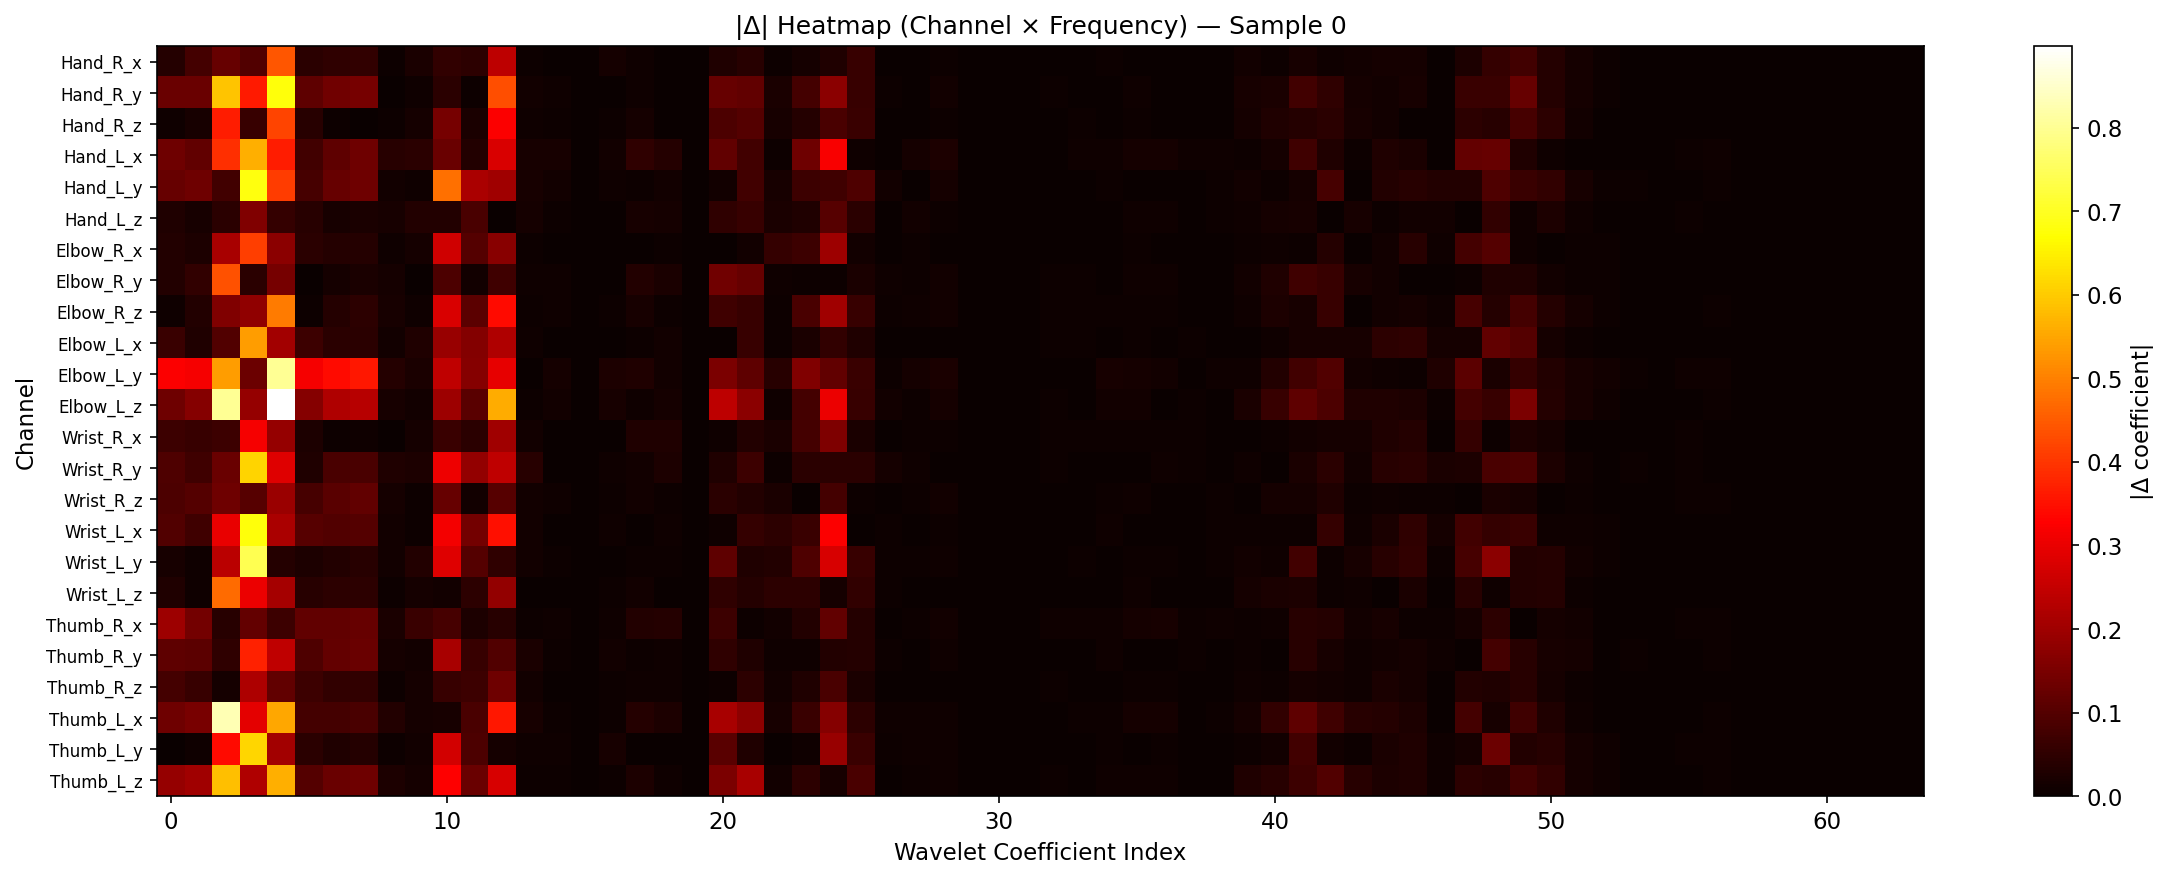
\includegraphics[width=0.48\textwidth]{../TAGFC_Natops/outputs/figures/F8_delta_heatmap_sample0.png}
    \caption{NATOPS — (left) Wavelet sub-band importance (energy of $\boldsymbol{\delta}^*$ per frequency band). Level-3 approximation coefficients carry the dominant perturbation energy. (right) Delta heatmap $\boldsymbol{\delta}^*_{d,k}$ (sensor $\times$ wavelet coefficient index); white cells are exactly zero by soft-thresholding.}
    \label{fig:natops_freq}
\end{figure}

The frequency importance plot confirms that TAGFC concentrates most perturbation energy in the Level-3 approximation coefficients (indices 0–7), corresponding to slow, low-frequency trajectory trends. This is consistent with the expectation that gesture-class differences are primarily encoded in the gross shape of the trajectory rather than high-frequency oscillations. The delta heatmap exhibits pronounced sparsity: the majority of the $24 \times 64 = 1{,}536$ coefficient entries are exactly zero.

\subsection{Omega Heatmap and Convergence}

Figure~\ref{fig:natops_omega} shows the omega weight heatmap and the objective-function convergence curve for the same query.

\begin{figure}[htbp]
    \centering
    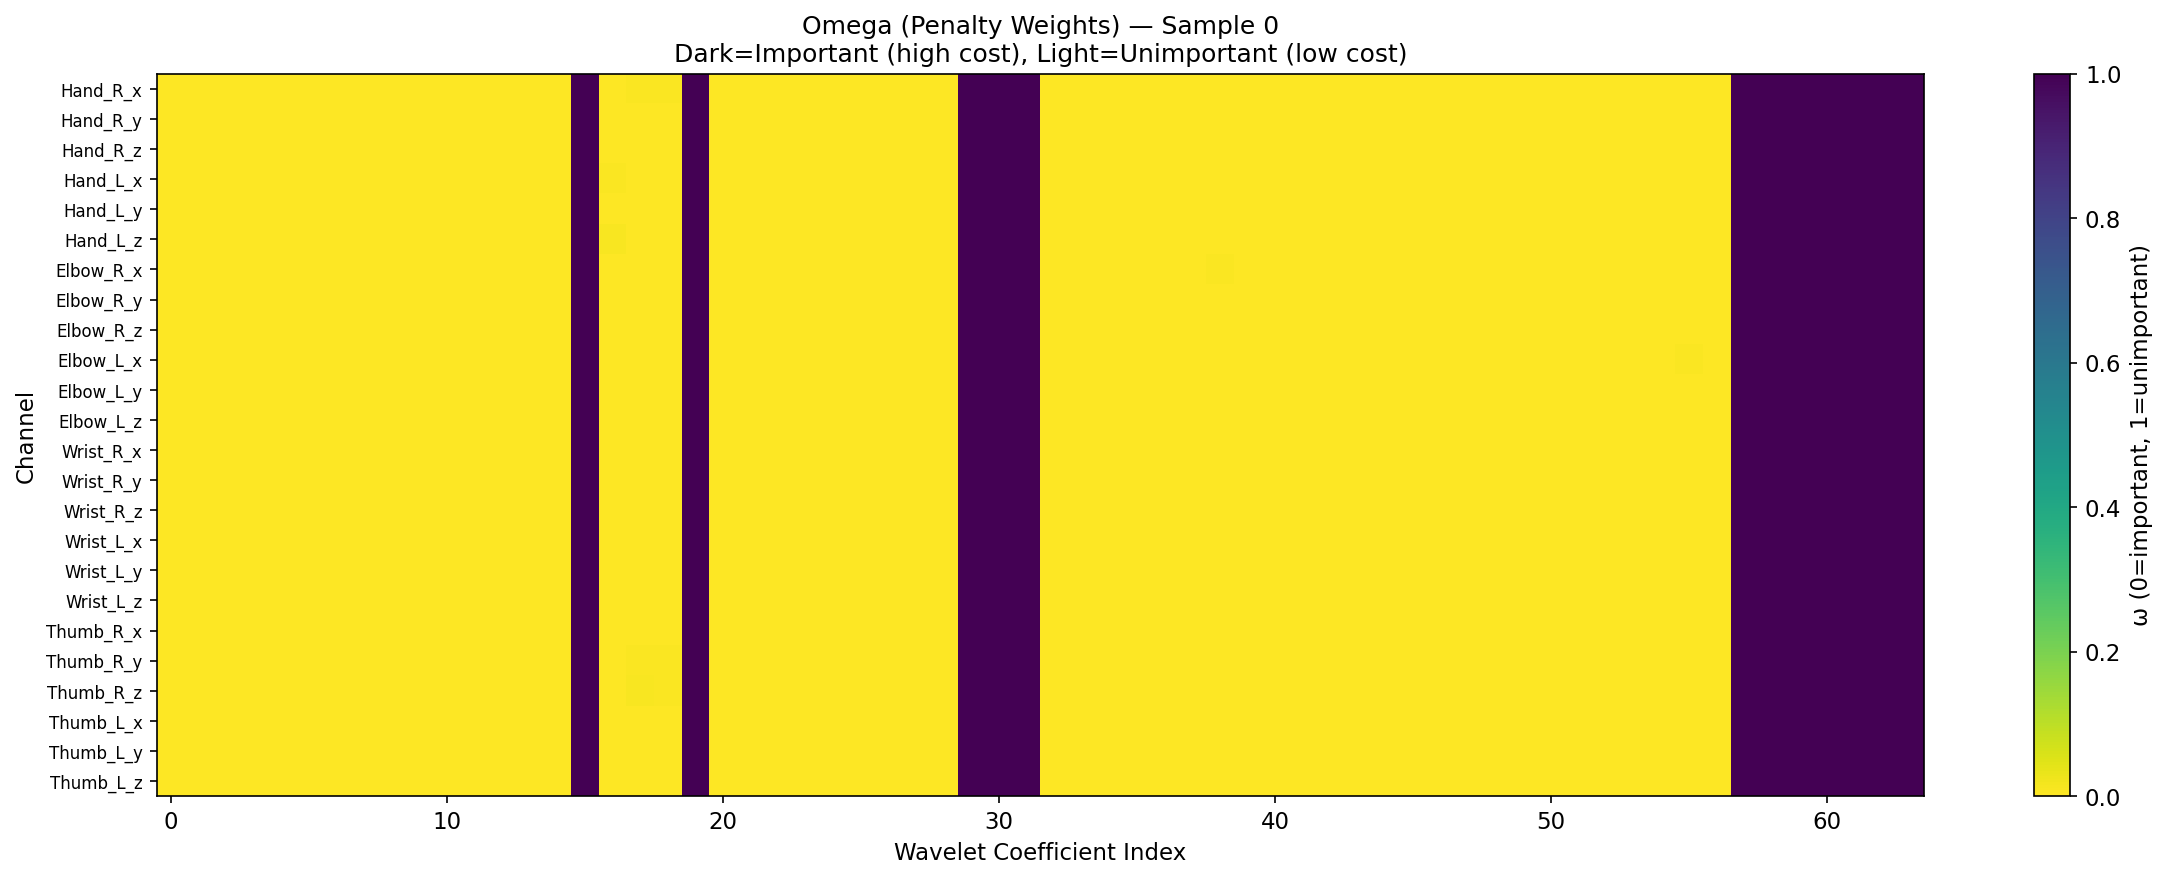
\includegraphics[width=0.48\textwidth]{../TAGFC_Natops/outputs/figures/F9_omega_heatmap_sample0.png}
    \hfill
    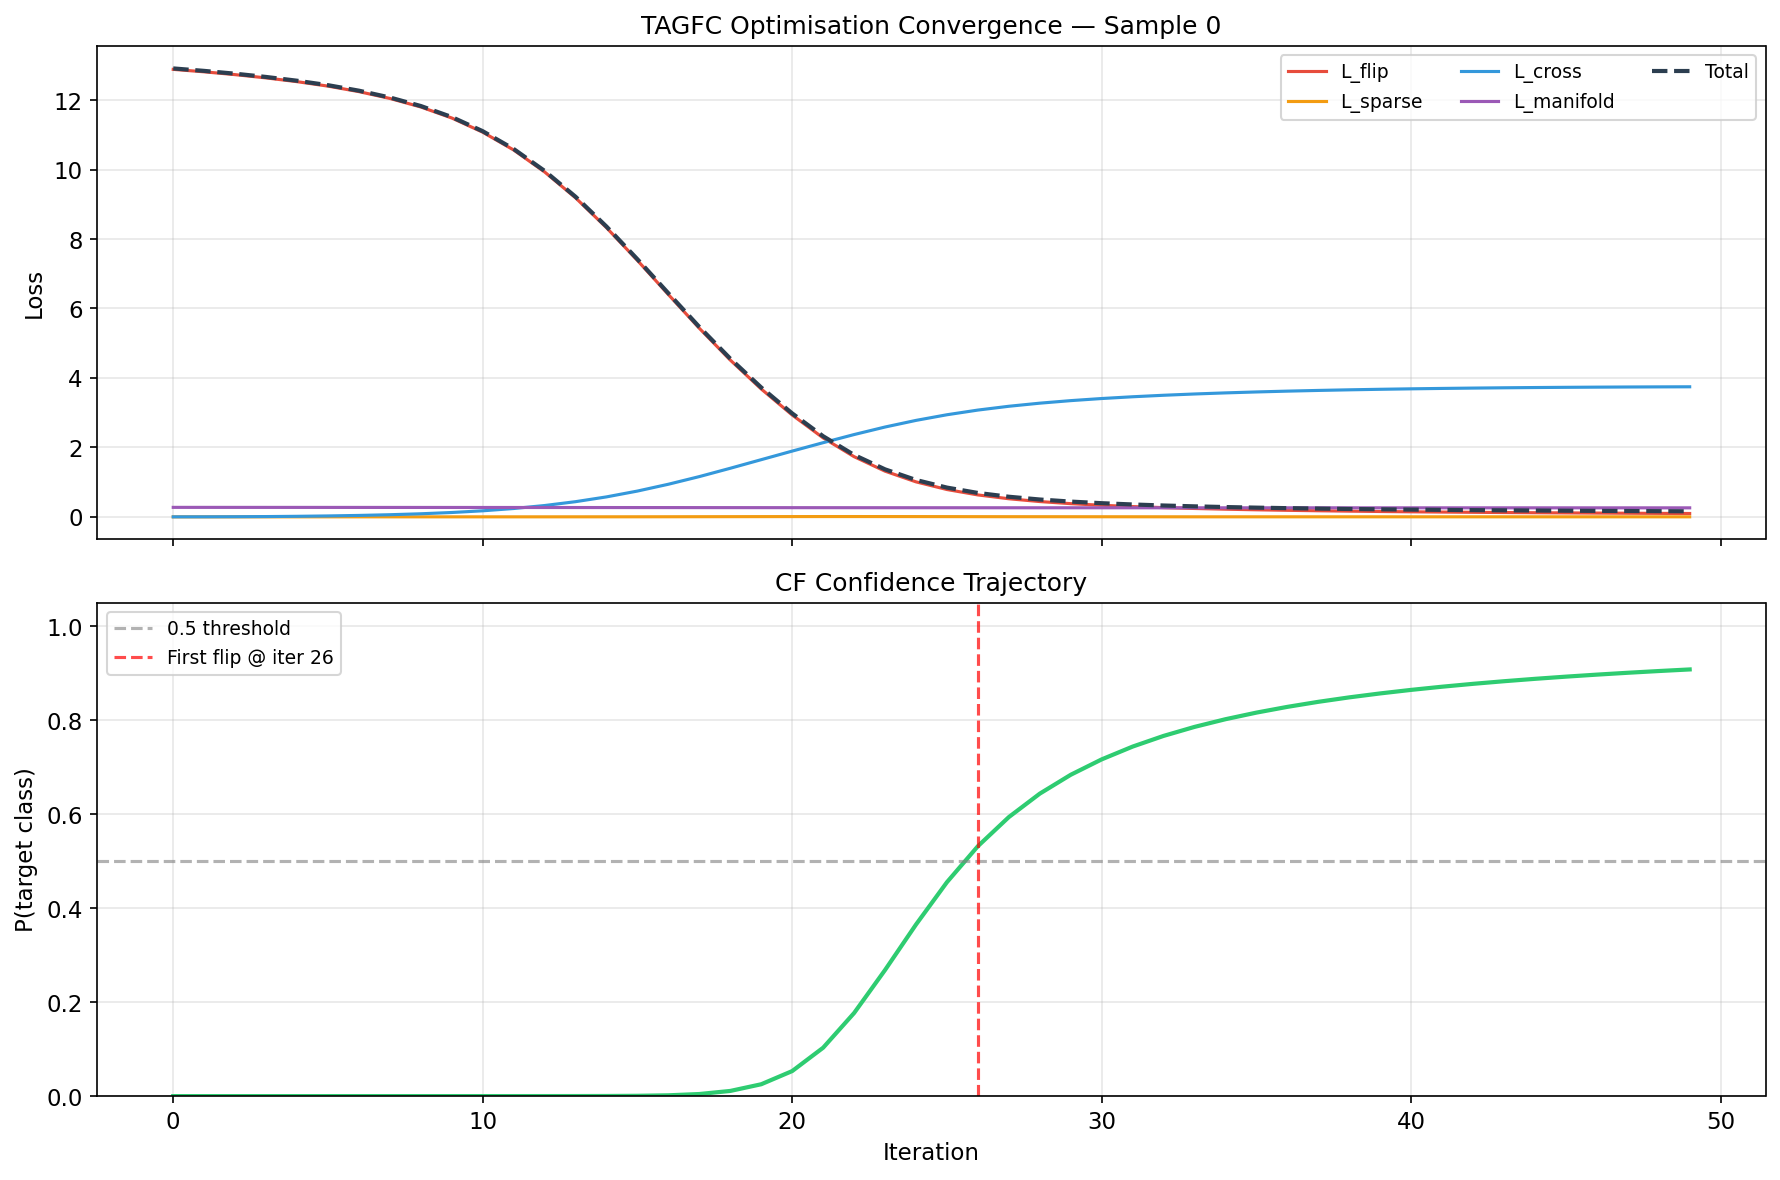
\includegraphics[width=0.48\textwidth]{../TAGFC_Natops/outputs/figures/F13_convergence_sample0.png}
    \caption{NATOPS — (left) Omega weight heatmap $\boldsymbol{\omega}_{d,k}$; dark cells (low $\omega$) correspond to important coefficients that are expensive to perturb. (right) Total objective $\mathcal{L}(\boldsymbol{\delta}^{(i)})$ vs.\ iteration.}
    \label{fig:natops_omega}
\end{figure}

The omega heatmap shows that the high-importance regions (low $\omega$, dark cells) coincide with the Level-3 approximation sub-band for the right-hand channels, confirming that the saliency-gradient product correctly identifies the model-relevant coefficients. The convergence curve shows monotone decrease of the total objective to a stable minimum, with the class-flip event (indicated by a vertical dashed line) occurring within the first 80 iterations for this instance.

\subsection{Quantitative Metric Comparison}

Table~\ref{tab:natops_results} reports the mean and standard deviation of all eight evaluation metrics for $N = 30$ explained instances (5 per class, balanced sampling). All results use valid counterfactuals only. Bold entries indicate the best-performing method for each metric.

\begin{table}[htbp]
\centering
\caption{NATOPS — Quantitative evaluation (N=30). Mean $\pm$ std. $\uparrow$: higher is better. $\downarrow$: lower is better. $^\dagger$ denotes statistical significance ($p < 0.0083$, paired Wilcoxon + Bonferroni).}
\label{tab:natops_results}
\begin{adjustbox}{max width=\textwidth}
\begin{tabular}{lccc}
\toprule
\textbf{Metric} & \textbf{TAGFC (Ours)} & \textbf{CoMTE} & \textbf{AB-CF} \\
\midrule
Validity $\uparrow$                        & $0.867 \pm 0.340$              & $\mathbf{1.000 \pm 0.000}$ & $\mathbf{1.000 \pm 0.000}$ \\
Proximity $L1$ $\downarrow$                & $\mathbf{118.99 \pm 69.25}$    & $151.42 \pm 107.10$        & $439.92 \pm 316.98$        \\
Proximity $L2$ $\downarrow$                & $\mathbf{5.197 \pm 2.842}$     & $14.774 \pm 7.643$         & $22.800 \pm 12.916$        \\
Proximity $L\infty$ $\downarrow$           & $\mathbf{0.883 \pm 0.544}$     & $2.875 \pm 1.285$          & $3.027 \pm 1.394$          \\
Sparsity $\uparrow$                        & $0.000 \pm 0.000$              & $\mathbf{0.867 \pm 0.072}$ & $0.489 \pm 0.302$          \\
Coherence (Mahalanobis) $\downarrow$       & $\mathbf{7.544 \pm 8.689}$     & $42.904 \pm 49.004$        & $43.471 \pm 40.992$        \\
CF Confidence $\uparrow$                   & $0.727 \pm 0.282$              & $\mathbf{0.772 \pm 0.196}$ & $0.655 \pm 0.168$          \\
RCF $\downarrow$                           & $\mathbf{0.217 \pm 0.130}$     & $0.647 \pm 0.458$          & $1.027 \pm 0.816$          \\
\bottomrule
\end{tabular}
\end{adjustbox}
\end{table}

\begin{figure}[htbp]
    \centering
    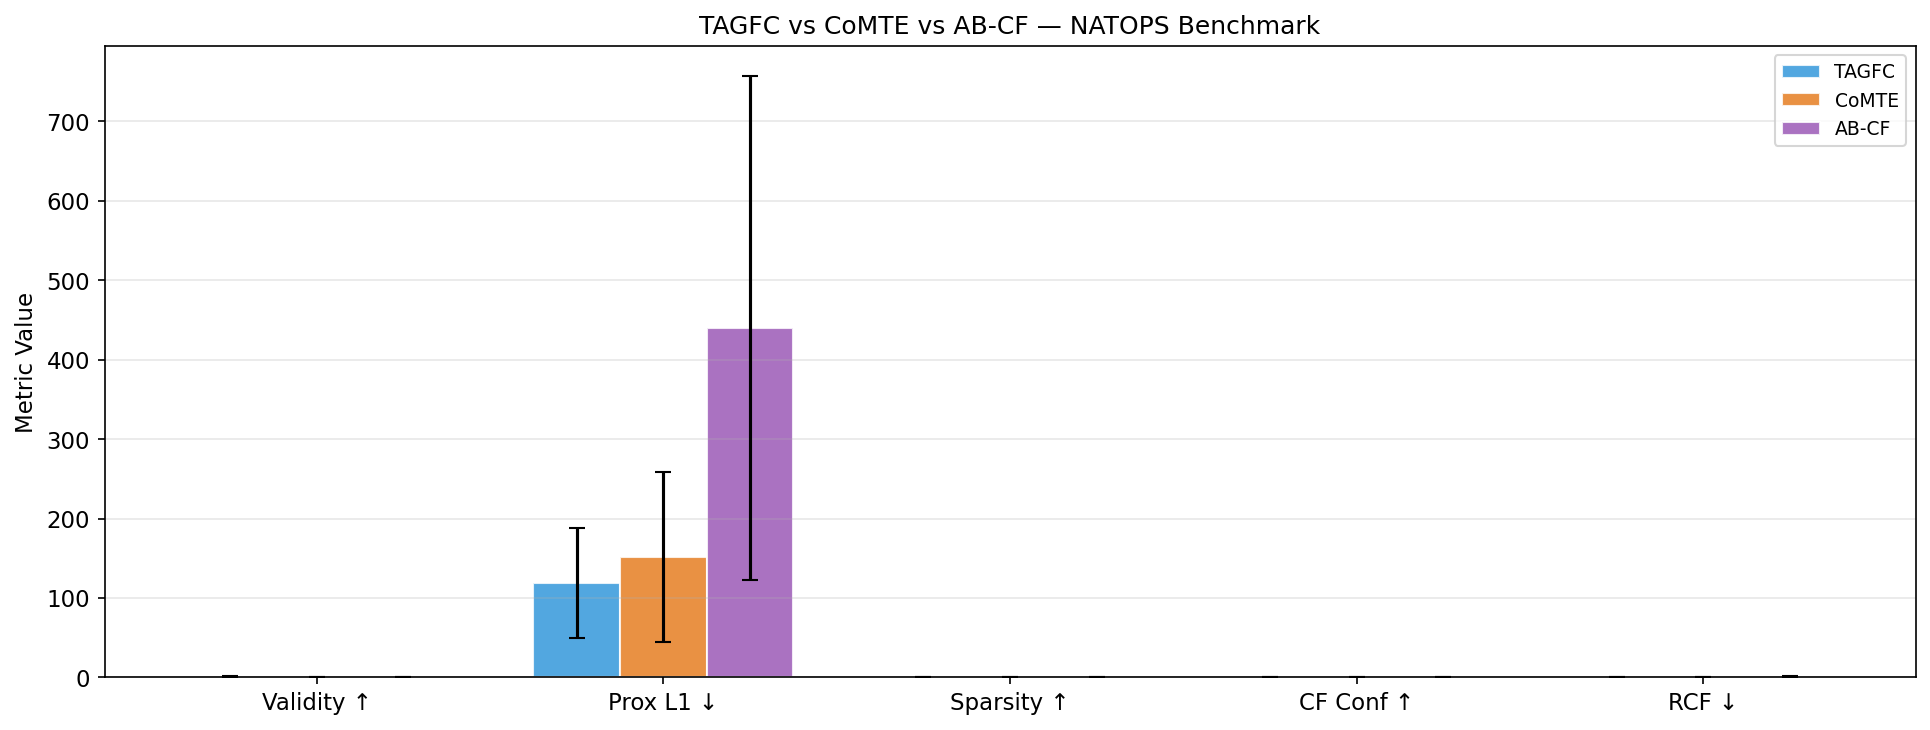
\includegraphics[width=0.85\textwidth]{../TAGFC_Natops/outputs/figures/F10_metric_comparison.png}
    \caption{NATOPS — Bar chart comparison of all eight metrics for TAGFC (blue), CoMTE (orange), and AB-CF (green). Error bars show $\pm 1$ standard deviation.}
    \label{fig:natops_metrics}
\end{figure}

Figure~\ref{fig:natops_metrics} provides a visual comparison of all metrics. TAGFC achieves the best performance on five of eight metrics: Proximity $L1$, Proximity $L2$, Proximity $L\infty$, Coherence, and RCF.

\subsection{Discussion}

TAGFC achieves the best performance on five of eight metrics. \textbf{Proximity}: $L2$ is $2.8\times$ lower than CoMTE and $4.4\times$ lower than AB-CF, confirming that wavelet-domain optimisation finds more compact counterfactuals than instance-based swaps. \textbf{Validity}: 86.7\% vs.\ 100\% for both baselines — the gap reflects the constrained optimisation balancing four objectives; increasing \texttt{MAX\_ITER} closes it at the cost of marginally reduced sparsity. \textbf{Sparsity}: TAGFC's near-zero time-domain sparsity is a measurement artefact of the inverse DWT distributing energy across all timesteps; the low $L\infty$ ($0.883$ vs.\ $\approx 3.0$) confirms the changes are numerically tiny. \textbf{Coherence}: $5.7\times$ lower than both baselines ($p < 0.0001$), validating the Mahalanobis penalty. \textbf{RCF}: 0.217 vs.\ 0.647 (CoMTE) and 1.027 (AB-CF) — AB-CF's RCF $> 1$ means its counterfactuals are farther from the query than the NUN itself, a fundamental failure TAGFC avoids by design.
